\documentclass[10pt,a4paper,twocolumn]{article}
\usepackage{amsmath}
\usepackage{amssymb}
\usepackage{graphicx}
\usepackage[a4paper]{geometry}
\geometry{vmargin={2cm,2cm},hmargin={1cm,1cm}}

\title{ANS-WINTER2010}
\date{2010.06.08}
\author{Damien Lebrun-Grandi\'e}

\newcommand\bs{\boldsymbol}
\newcommand\bx{\bs{x}}
\newcommand\bn{\bs{\nabla}}

\begin{document}

%%%%%%%%%%%%%%%%%%%%%
%%%HEADERS
\noindent
\begin{tabular}{|p{9cm}|}
  \hline
  \begin{center}
    \textbf{Method of Manufactured Solutions for a 2D Neutronics/Heat Conduction Test Case with Adaptive Multimesh hp-FEM} \\
    Damien Lebrun-Grandi\'e,%$^{a}$,
    Jean Ragusa,%$^{a}$, 
%    Pavel Solin$^{b}$, 
    Bruno Turcksin \\%$^{a}$, 
%    Ondrej Certik$^{b}$ \\
    \emph{Department of Nuclear Engineering, Texas A\&M University, College Station, TX 77843-3133, USA} \\
%    \emph{$^{b}$Department of Mathematics and Statistics, University of Nevada, Reno, NV 89557-0208, USA} \\
    lebrungd@neo.tamu.edu
  \end{center} \\
  \hline
\end{tabular}

%%%%%%%%%%%%%%%%%%%%%
%%%BODY
\section*{INTRODUCTION}
Once upon a time...

Typically, the accuracy and convergence of numerical models are established by using simplified problems for which analytical solutions are available. For time-dependent coupled multiphysics problems, analytical solutions are more difficult to obtain and we need to resort to the Method of Manufactured Solutions (MMS) \cite{roache2002}. The MMS can be used to analyze and prove code correctness.

The basic philosophy behind MMS is that an exact solution Uref with enough smoothness in space and time is chosen and substituted into the PDE to obtain a suitable forcing function (i.e., right-hand-side of the PDE) that is employed in the numerical simulation. Therefore, the numerically obtained values can be compared to the exact ones, providing a measure of the error. This procedure can be applied to nonlinear and coupled physics problems and is an useful tool for code verification purposes.

A new C++ library for adaptive hp-FEM currently is currently under active development at the University of Nevada, Reno \cite{solin2010}.   The exponential convergence makes the method a very attractive choice for solving multiphysics PDE systems.  In collaboration with the hp-FEM group at Reno, Texas A\&M University is



\section*{THEORY}
Method of Manufactured Solutions to verify convergence to exact solutions


\subsection*{Governing equations}
2D nonlinear transient problem involving neutronics and heat conduction

%%%%%%%%%%%%%%%%%%%%%%%%%%%%%%%%%%%%%%%%%%%%%%%%%%%%%%%%%%%%%%%%%%%%%%%%%%%%%%%%
%%%%  HEAT CONDUCTION
%\subsection*{$\rightarrow$Heat conduction}
Let us solve the following equation for the temperature $T(\bx, t)$
\begin{align}
  \rho c_p \frac{\partial T}{\partial t} 
  - \nabla\cdot(k(T) \nabla T) 
  - \kappa \Sigma_{f} \phi(\bx,t)&  \nonumber \\
  - Q_T(\bx,t) &= 0 \label{heatcond_eq}
\end{align}
on a rectangular domain $\Omega$ with a homogeneous (zero) Dirichlet boundary condition $T(\bx,t) = 0$ on $\partial\Omega$, where the thermal conductivity $k$ depends on the temperature $T$
\begin{align}
  k(T) = k(T_{ref}) + \left. \frac{\partial k}{\partial T}\right|_{ref} \left( T - T_{ref} \right)
\end{align}

$Q_T$ is the extraneaous temperature source and will be determined by the choice of the exact solution in the MMS procedure.  This is a function of space and time a priori.

The weak formulation of the time discretized (implicit Euler) heat conduction problem is derived in the standard way, by first multiplying the equation \eqref{heatcond_eq} with the test functions $u_{i}$ and then integrating over the domain $\Omega$
\begin{align}
  \int_{\Omega} \rho c_p \frac{T^{n+1}-T{^n}}{\tau} u_i d\bx 
  - \int_{\partial\Omega} k(T^{n+1}) \nabla T^{n+1} u_i \cdot \bs{n} d\bx&  \nonumber \\
  + \int_{\Omega} k(T^{n+1}) \nabla T^{n+1} \cdot \nabla u_i d\bx
  - \int_{\Omega} \kappa_1 \Sigma_{f1} \phi_1^{n+1} u_i d\bx& \nonumber \\
  - \int_{\Omega} Q_T^{n+1} u_i d\bx = 0& \label{heatcond_wf}
\end{align}
(constant time step $\tau$)

%%%%%%%%%%%%%%%%%%%%%%%%%%%%%%%%%%%%%%%%%%%%%%%%%%%%%%%%%%%%%%%%%%%%%%%%%%%%%%%%
%%%%  NEUTRONICS
%\subsection*{$\rightarrow$Neutronics}
The neutron flux $\phi(\bx,t)$ is described by means of a simple one-group neutron diffusion equation
\begin{align}
  \frac{1}{v} \frac{\partial\phi}{\partial t} 
  - \nabla\cdot(D \nabla \phi) 
  + \Sigma_{a}(T) \phi 
  - \nu \Sigma_{f} \phi_1& \nonumber \\
  - Q(\bx,t) &= 0 \label{neutron_eq}
\end{align}

Doppler feedback is accounted in the model through the removal cross section $\Sigma_{a}$, which is affected by temperature variations.
\begin{align}
  \Sigma_{a}(T) = \Sigma_{a}(T_{ref}) 
  + \left. \frac{\partial \Sigma_{a}}{\partial \sqrt{T}}\right|_{ref} 
    \left( \sqrt{T} - \sqrt{T_{ref}} \right)
\end{align}

The forcing function $Q$ in the equation \eqref{neutron_eq} will be determined later when choosing the exact solutions, and substituting these into the governing equations.

Finally, with the homogeneous zero Dirichlet condition, the weak formulation of the neutronics problem reads
\begin{align}
  \int_{\Omega} \frac{1}{v} \frac{\phi^{n+1}-\phi{^n}}{\tau} u_i d\bx 
  - \int_{\partial\Omega} D \nabla \phi^{n+1} u_i \cdot \bs{n} d\bx& \nonumber \\
  + \int_{\Omega} D \nabla \phi^{n+1} \cdot \nabla u_i d\bx 
  + \int_{\Omega} \Sigma_{a}(T^{n+1}) \phi^{n+1} u_i d\bx& \nonumber \\
  - \int_{\Omega} \nu \Sigma_{f} \phi^{n+1} u_i d\bx 
  - \int_{\Omega} Q^{n+1} u_i d\bx = 0&
\end{align}



\subsection*{Newton's method}
For fixed time level $n$ we will solve the time independent nonlinear problem for the temperature $T^{n}$ and the neutron flux $\phi^{n}$ by means of the Newton's Method.

Let $\bs{Y}^n = (y_1^n,y_2^n,...,y_N^n)^T$ be the vector of unknown coefficients so that we have

At each Newton iteration $k$ we solve
\begin{align}
  \bs{Y}_{k+1}^{n} = \bs{Y}_{k}^{n} 
  - \bs{J}^{-1}(\bs{Y}_{k}^{n}) \bs{F}(\bs{Y}_{k}^{n})
\end{align}
or
\begin{align}
  \bs{J}(\bs{Y}_{k}^{n}) \delta\bs{Y}_{k}^{n} = - \bs{F}(\bs{Y}_{k}^{n}) \label{newton}
\end{align}
where $\bs{Y}_{k+1}^{n} = \bs{Y}_{k}^{n} + \delta\bs{Y}_{k}^{n}$, $n$ and $k$ being indices for time and Newton iterations respectively.

All we need to do is to provide the code with the Jacobian matrix $\bs{J}^{n}=\bs{J}(\bs{Y}^{n})=D\bs{F}^{n}/D\bs{Y}^{n}$
and the residual vector $\bs{F}^{n}=\bs{F}(\bs{Y}^n)=\bs{0}$.

\subsection*{Manufactured Solution}
Choice of
\begin{align}
  T(x,y,t) = 
  C_T \left(1+\tanh(r_T t)\right)
  \sin\left(\frac{\pi x}{L_X}\right)
  \sin\left(\frac{\pi y}{L_Y}\right)
\end{align}
and
\begin{align}
  \phi(x,y,t) = 
  C_F \left(1+\exp(r_F t)\right)
  \sin\left(\frac{\pi x}{L_X}\right)
  \sin\left(\frac{\pi y}{L_Y}\right)
  \frac{x}{L_X}
  \frac{y}{L_Y}
\end{align}



\section*{RESULTS}
%%%%%%%%%%%%%%%%%%%%%%%%%%%%%%%%%%%%%%%%%%%%%%%%%%%%%%%%%%%%%%%%%%%%%%%%%%%%%%%%
%%%%  hp-FEM
The problem described above was solved using Hermes2D\footnote{http://hpfem.org/hermes2d/}, a new open-source C++ library for development adaptive $hp$-FEM solvers for PDEs, currently under active development at University of Nevada, Reno.  We took advantage of the adaptive $hp$-FEM algorithms \cite{solin2010} from Hermes2D to solve the two physics on individual meshes.

%refine the mesh element or increase the polynomial degree

%%%%%%%%%%%%%%%%%%%%%%%%%%%%%%%%%%%%%%%%%%%%%%%%%%%%%%%%%%%%%%%%%%%%%%%%%%%%%%%%
%%%%  MMS
%\subsection*{Manufactured Solution}
The following choice for $\phi(\bx,t)$ and $T(\bx,t)$ was made
\begin{align}
  \left\{ \begin{array}{l}
      \phi(x,y,t) = C_\phi \left(1+\exp(r_\phi t)\right) \sin\left(\frac{\pi x}{L_X}\right) \sin\left(\frac{\pi y}{L_Y}\right) \frac{x}{L_X} \frac{y}{L_Y} \\
      T(x,y,t) = C_T \left(1+\tanh(r_T t)\right) \sin\left(\frac{\pi x}{L_X}\right) \sin\left(\frac{\pi y}{L_Y}\right)
  \end{array} \right.
\end{align}
and a script was written to perform the symbolic calculation of the forcing terms $Q(\bx,t)$ and $Q_T(\bx,t)$ so that the MMS can be used to verify the convergence to the exact solution when solving the 

The solution $\phi(x,y)$ at time level $t=0.1 \mbox{sec}$ for adaptive $h$-FEM with quadratic quadrilateral elements (p=2) is shown in Fig. \ref{sol_temp}.  Since the exact solution is available, both the estimated error (comparing solution on coarse mesh with solution on finer mesh at each adaptivity step) and the exact error were computed.  The estimated error is slightly less than the exact one, but converges quickly to the exact error during adaptivity to become virtually identical (0.000186 \% for the estimated error versus 0.000187 \% in the solution for $\phi(x,y)$ in Fig. \ref{sol_temp}).
\begin{figure}
  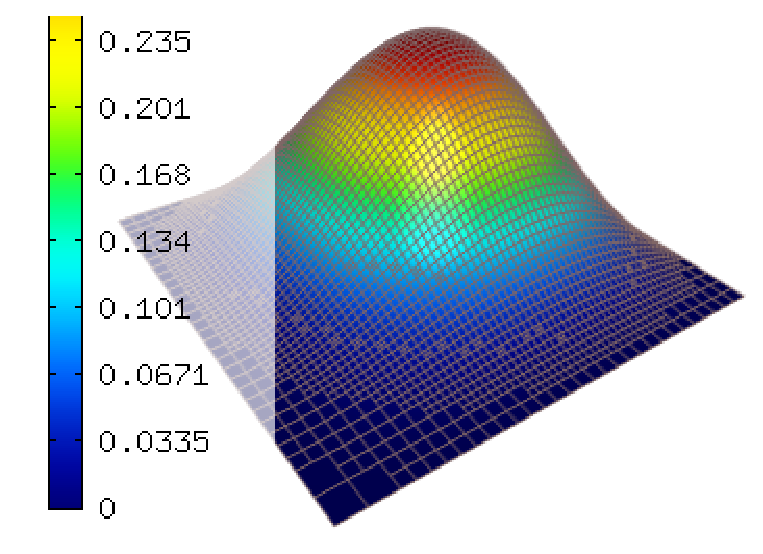
\includegraphics[width=0.5\textwidth]{figures/solution_T}
  \caption{Solution for $\phi(x,y)$ at time level $t=0.1 \mbox{sec}$ using adaptive $h$-FEM and $p=2$.  This contains 60353 DOFs and has a relative error 0.00019 \%.}
  \label{sol_temp}
\end{figure}

The problem was solved using both $h$-adaptivity with linear ($p=1$) as well as quadratic ($p=2$) quadrilateral elements and $hp$-adaptivity.  Fig. \ref{err_conv} shows the convergence rate for the temperature $T(x,y)$ at time level $t=0.1 \mbox{sec}$ in terms of the size of the number of degrees of freedom (DOFS).
\begin{figure}
  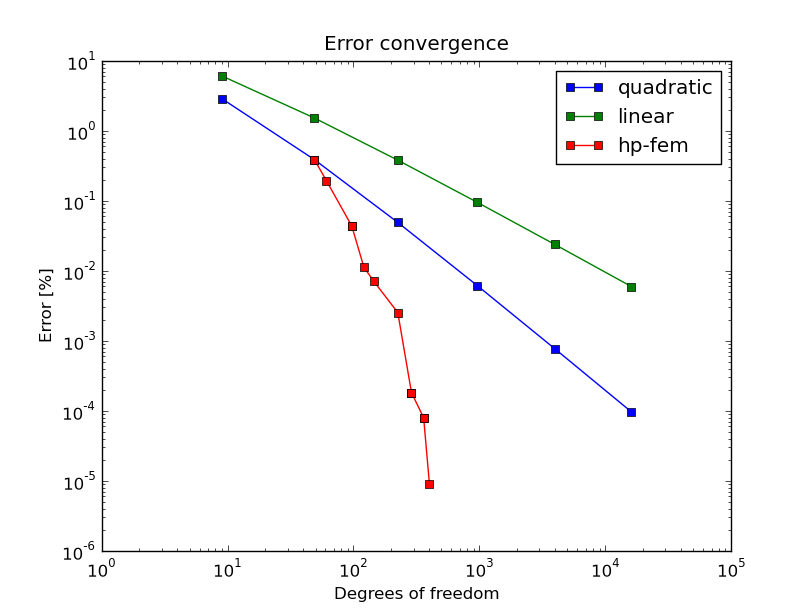
\includegraphics[width=0.5\textwidth]{figures/exact_err_conv}
  \caption{Convergence comparison of adaptive $hp$-FEM with adaptive $h$-FEM on linar ($p=1$) and quadratic ($p=2$) finite elements.  The error plotted is the exact relative error in norm $L_2$ for the temperature $T(x,y)$ at time level $t=0.1 \mbox{sec}$.}
  \label{err_conv}
\end{figure}

The error ploted is the relative error in $L_2$ norm, between the numerical results $T$ and the analytical solution $T_{exact}$.  It is computed using
\begin{align}
  e = \frac{ \|T-T_{exact}\|_{L_2} }{ \|T_{exact}\|_{L_2} }
\end{align}

As we may see on the figure, the convergence graphs of adaptive $h$-FEM show the slopes in $-p/d$ on the log-log scale predicted by the theory, and adaptive $hp$-FEM does reach exponential convergence.


\section*{CONCLUSION}
\vspace{-4mm}
Adaptive $hp$-FEM has been efficiently applied to a two-dimensional nonlinear coupled neutronics/heat conduction problem.  The convergence of $hp$-FEM to the exact solution was found to be exponential on a log-log scale (whereas $h$-FEM converges only algebraically).
%
Future work will include (a) treatment of multi-group neutron diffusion with delayed neutron precursors and (b) implementation of higher-order methods for the time discretization.



\section*{Acknowledgments}
The authors are grateful for 



\begin{thebibliography}{99}
\bibitem{roache2002}  P. J. ROACHE,
  ``Code Verification by the Method of Manufactured Solutions'', 
  \emph{ASME J. of Fluids Eng.},
  \textbf{124}, 1, 4-10 (2002)
\bibitem{solin2010} P. SOLIN, D. ANDRS, J. CERVENY, M.SIMKO,
  ``PDE-Independent Adaptive hp-FEM Based on Hierarchic Extension of Finite Element Spaces'',
  \emph{J. Comput. Appl. Math.},
  \textbf{233}, 1374-1394 (2010)
\end{thebibliography}

%\bibliographystyle{genetics} 
%\bibliography{references}

\end{document}
